\documentclass[xcolor=table,dvipsnames,svgnames,aspectratio=169,fontset=windows]{ctexbeamer}
% 可以通过 fontset=macnew / fontset=ubuntu / fontset=windows 选项切换字体集
\usepackage{tikz}
\usepackage[normalem]{ulem}
\usetikzlibrary{arrows}
\usepackage{amsmath}
\usepackage{mflogo}
\usepackage{graphicx}
\usepackage{ccicons}
\usepackage{hologo}
\usepackage{colortbl}
\usepackage{shapepar}
\usepackage{hyperxmp}
\usepackage{booktabs}
\usepackage{qrcode}
\usepackage{listings}
\usepackage{tipa}
\usepackage{multicol}
\usepackage{datetime2}
\usepackage{fontawesome5}
\usepackage{hyperref}
\usepackage{enumitem}
\usepackage[backend=biber,style=gb7714-2015]{biblatex}
\addbibresource{thesis.bib}
\graphicspath{{figures/}}
\hypersetup{
  pdfsubject = {上海交通大学图书馆专题培训讲座},
  pdfauthor = {Alexara Wu},
  pdfcopyright = {Licensed under CC-BY-SA 4.0. Some rights reserved.},
  pdflicenseurl = {http://creativecommons.org/licenses/by-sa/4.0/},
  unicode = true,
  psdextra = true,
  pdfdisplaydoctitle = true
}

\pdfstringdefDisableCommands{
  \let\\\relax
  \let\quad\relax
  \let\hspace\@gobble
}
\renewcommand{\TeX}{\hologo{TeX}}
\renewcommand{\LaTeX}{\hologo{LaTeX}}
\newcommand{\BibTeX}{\hologo{BibTeX}}
\newcommand{\XeTeX}{\hologo{XeTeX}}
\newcommand{\pdfTeX}{\hologo{pdfTeX}}
\newcommand{\LuaTeX}{\hologo{LuaTeX}}
\newcommand{\MiKTeX}{\hologo{MiKTeX}}
\newcommand{\MacTeX}{Mac\hologo{TeX}}
\newcommand{\beamer}{\textsc{beamer}}
\newcommand{\XeLaTeX}{\hologo{Xe}\kern-.13em\LaTeX{}}
\newcommand{\pdfLaTeX}{pdf\LaTeX{}}
\newcommand{\LuaLaTeX}{Lua\LaTeX{}}
\def\TeXLive{\TeX{} Live}
\let\TL=\TeXLive
\newcommand{\SJTUThesis}{\textsc{SJTUThesis}}
\newcommand{\SJTUThesisVersion}{1.1.0}
\newcommand{\SJTUThesisDate}{2023/3/24}
\newcommand{\SJTUBeamer}{\textsc{SJTUBeamer}}
\newcommand{\SJTUBeamerVersion}{3.0.0}
\newcommand{\SJTUBeamerDate}{2022/11/22}
\newcommand\link[1]{\href{#1}{\faLink}}
\newcommand\pkg[1]{\texttt{#1}}
\def\cmd#1{\texttt{\color{structure}\footnotesize $\backslash$#1}}
\def\env#1{\texttt{\color{structure}\footnotesize #1}}
\def\cmdxmp#1#2#3{\small{\texttt{\color{structure}$\backslash$#1}\{#2\}
\hspace{1em}\\ $\Rightarrow$\hspace{1em} {#3}\par\vskip1em}}
\lstset{
  language=[LaTeX]TeX,
  basicstyle=\ttfamily\footnotesize,
  tabsize=2,
  keywordstyle=\bfseries\ttfamily\color{cprimary},
  commentstyle=\sl\ttfamily\color[RGB]{100,100,100},
  stringstyle=\ttfamily\color[RGB]{50,50,50},
  extendedchars=true,
  breaklines=true,
}

\usetheme[maxplus]{sjtubeamer}
\author{汇报人:侯力广}
\date{\the\year \,.\the\month \,}
\subject{LaTeX, 论文排版, SJTUThesis}
\title[基于网格的NM不等式约束优化算法]
{\textbf{基于网格的NM不等式约束优化算法}} 

%=================================================================
%==================================================================

\begin{document}

\maketitle
\begin{frame}{引言}
  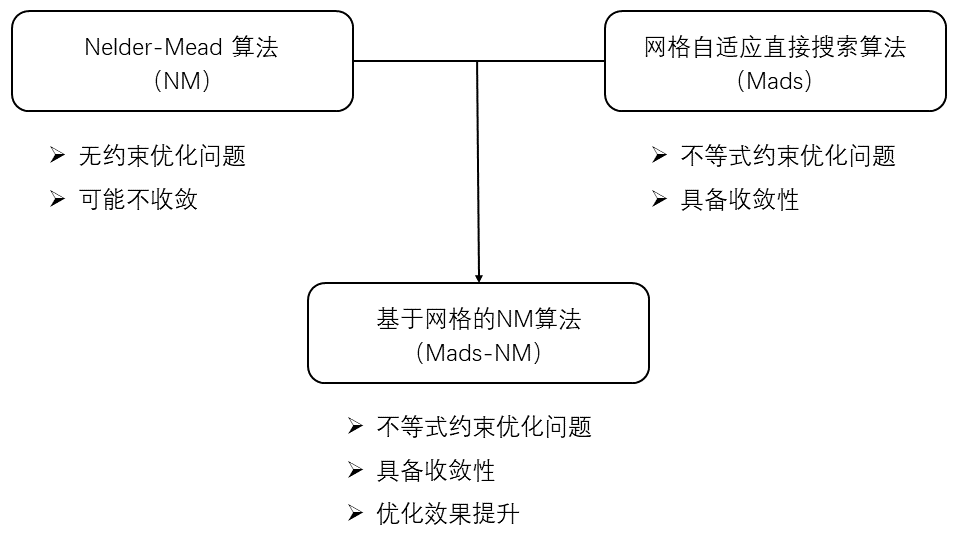
\includegraphics[width=0.8\textwidth,height=0.8\textheight]{summary-c.png}
\end{frame}

%-----------------------------------------------------------------------

\begin{frame}{目录}
  \tableofcontents[hideallsubsections]
\end{frame}

%-----------------------------------------------------------------------

\section{NM无约束优化算法}
\begin{frame}{NM-基本概念}
  对于无约束优化问题$\underset{x\in\mathrm{R}^n}{\mathrm{min} } f(x)$,
  \begin{itemize}[itemsep= 15 pt,topsep = 15 pt,leftmargin= 20 pt]
    \item $\spadesuit\quad$$x,y\in\mathbb{R}^n$,若$f(x)<f(y)$,称$x$控制$y$,记作$x \prec y$.
    \item $\spadesuit\quad$$ \operatorname{Older}(x, y)=\left\{\begin{array}{cl}
      \quad\; x & \qquad\text {若 } x \text { 在 } y \text { 之前生成}\\
      \quad\; y & \qquad\text {其他 }
      \end{array}\right.$\\
    \item $\spadesuit\quad$$\operatorname{Best}(x, y)=\left\{\begin{array}{cl}
      x & \text {若 } x \prec  y \\
      y & \text {若 } y \prec  x \\
      \operatorname{Older}(x, y) & \text {若 } f(x)=f(y)
      \end{array}\right.$
  \end{itemize}
\end{frame}

\begin{frame}{NM-基本概念}
  \begin{columns}
  \column{0.6\linewidth}
  $\mathbb{Y}=\{y^0,y^1,\cdots,y^n\}$是$\mathrm{R}^n$中的一个有序单纯形
    $$\begin{array}{ll}
      x^c=\frac{1}{n}\sum_{i=0}^{n-1}y^i\quad\quad&\text{中心}\vspace{8pt}\\
      x^r=x^c+(x^c-y^n)\quad\quad&\text{反射点}\vspace{8pt}\\
      x^e=x^c+2(x^c-y^n)\quad\quad&\text{延长点}\vspace{8pt}\\
      x^{oc}=x^c+\frac{1}{2}(x^c-y^n)\quad\quad&\text{外缩点}\vspace{8pt}\\
      x^{ic}=x^c-\frac{1}{2}(x^c-y^n)\quad\quad&\text{内缩点}\vspace{8pt}\\
      \gamma=\frac{1}{2}\quad\quad&\text{收缩参数}\\
    \end{array}$$
  \column{0.4\linewidth}
  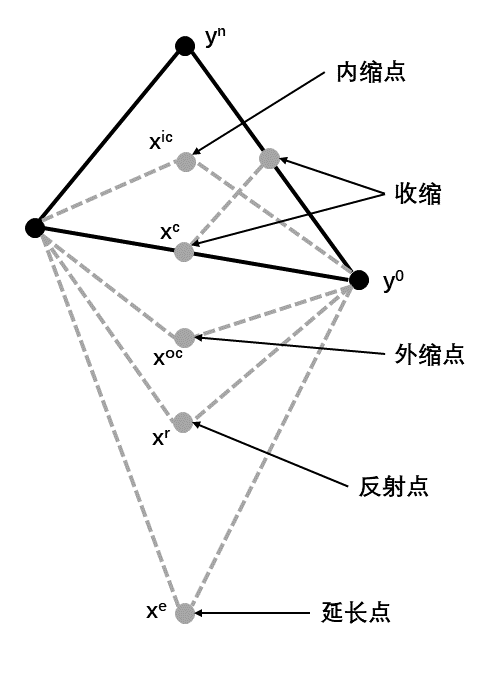
\includegraphics[width=0.88\textwidth,height=0.9\textheight]{nm-4-c.png}
  \end{columns}
\end{frame}

\begin{frame}{NM-算法思路}
  \begin{columns}
    \column{0.33\linewidth}
    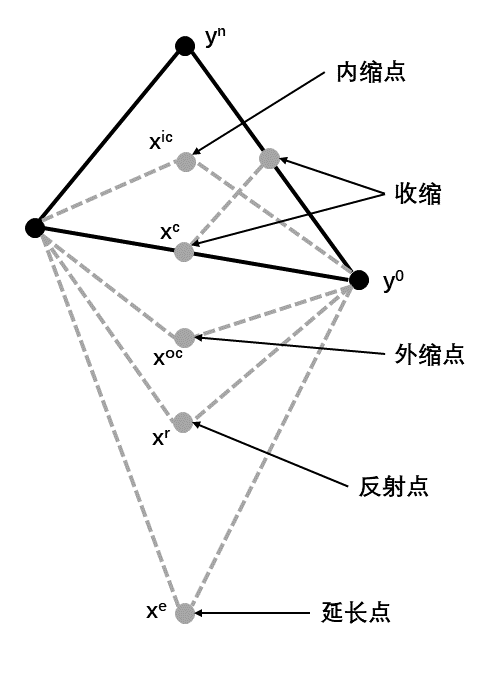
\includegraphics[width=1.08\textwidth,height=0.9\textheight]{nm-4-c.png}
    \column{0.7\linewidth}
    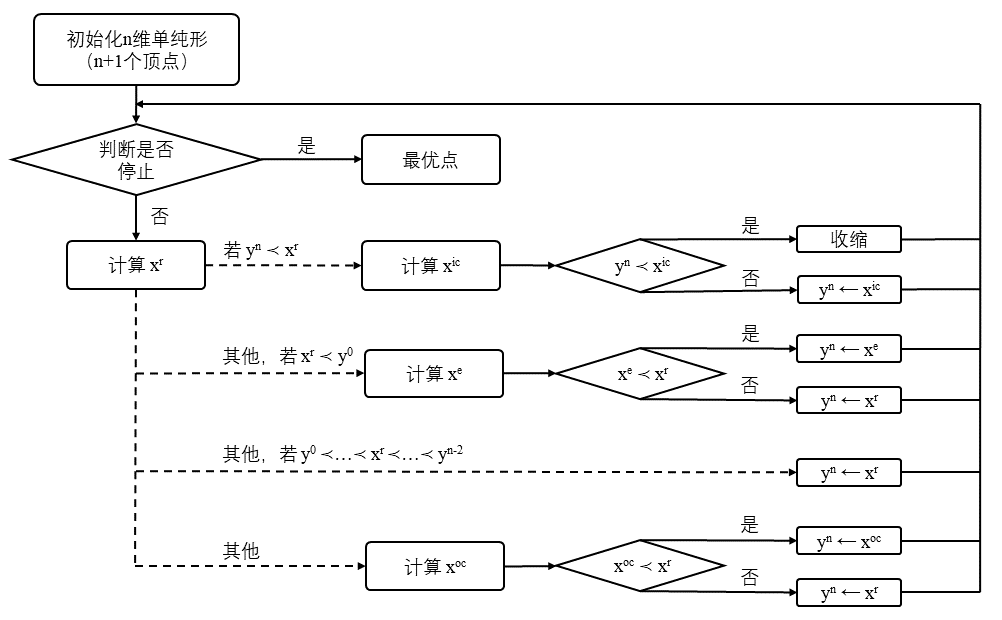
\includegraphics[width=\textwidth,height=0.85\textheight]{nm-3-c.png}
  \end{columns}
\end{frame}
%-----------------------------------------------------------------------
\section{Mads不等式约束优化算法}
\begin{frame}{Mads-基本概念}
  对于不等式约束优化问题$\quad\begin{aligned}&\underset{x\in X\subset\mathrm{R}^n}{\mathrm{min} } f(x)\\&s.t.\quad c(x)\leq 0\\\end{aligned}$,
  \begin{itemize}[itemsep= 15 pt,topsep = 15 pt,leftmargin= 20 pt]
    \item $\spadesuit\quad$ $f:X\mapsto\mathrm{R}\cup\infty$ 且$c:X\mapsto(\mathrm{R}\cup\infty)^m$
    \item $\spadesuit\quad$ 渐进障碍法(PB)通过违约函数寻找可行域内最优点\\$$h(x)=\left\{\begin{array}{ll}
      \sum_{j \in J}\left(\max \left\{c_{j}(x), 0\right\}\right)^{2} & \text {若 } x \in X \\
      \infty & \text {其他 }
      \end{array}\right.$$\\
  \end{itemize}
\end{frame}

\begin{frame}{Mads-基本概念}
  \begin{columns}
    \column{0.5\linewidth}
    Mads的核心步骤为:搜索-轮询 \\
    $~$\\
    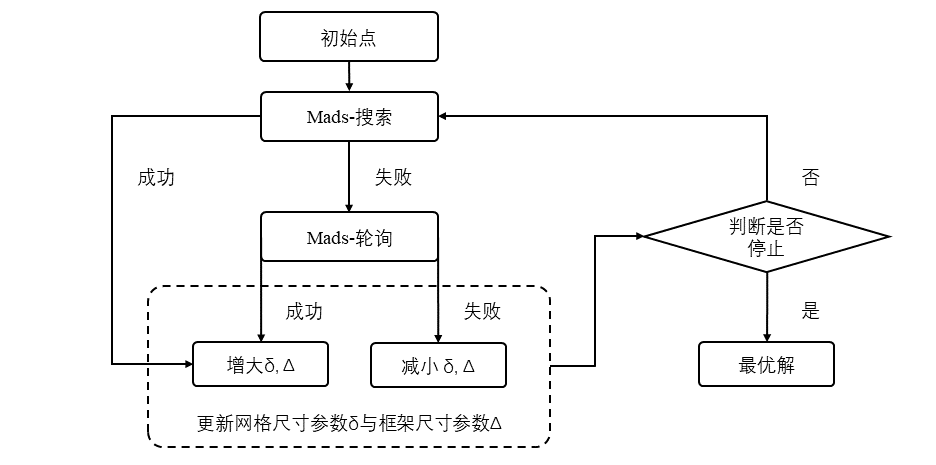
\includegraphics[width=1\textwidth,height=0.55\textheight]{mads-2-c.png}
    \column{0.5\linewidth}
    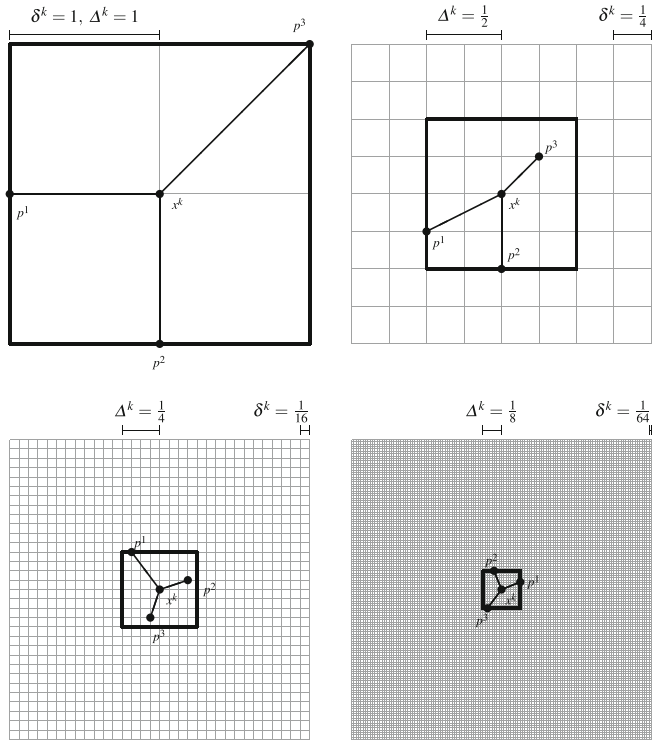
\includegraphics[width=0.8\textwidth,height=0.8\textheight]{mads-3.png}
  \end{columns}
\end{frame}

\begin{frame}{Mads-算法思路}
    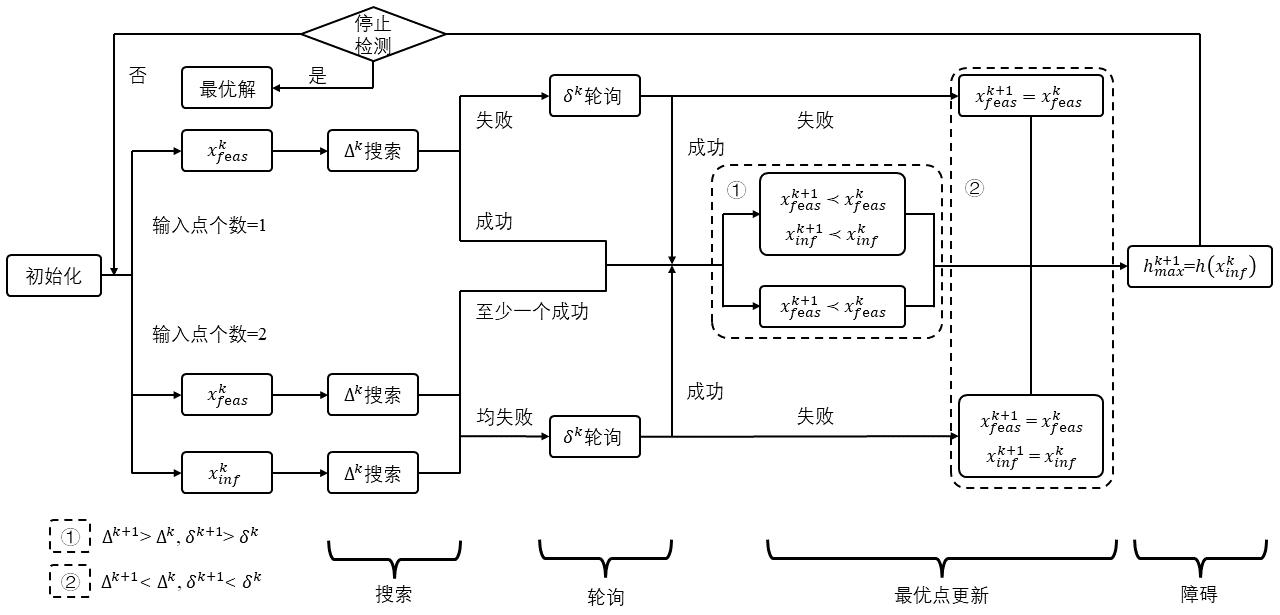
\includegraphics[width=0.95\textwidth,height=0.85\textheight]{mads-5-c.png}
\end{frame}


\begin{frame}{Mads-收敛性分析}
  如果测试点序列属于一个有界集,且更新方向集合足够丰富,则存在一个聚点$x^*$:
  \begin{itemize}[itemsep= 10 pt,topsep = 15 pt,leftmargin= 20 pt]
    \item $\bullet\quad$若$x^*$可行,则$x^*$在可行域$\Omega$的每个超切线方向$d$上,广义Clarke方向导数$f^{o}(x^*;d)$是非负的;
    \item $\bullet\quad$若$x^*$不可行,则$x^*$在集合$X$的每个超切线方向$d$上,广义Clarke方向导数$h^{o}(x^*;d)$是非负的。
  \end{itemize}
\end{frame}

%----------------------------------------------------------------------
\section{Mads-NM不等式约束优化算法}
\begin{frame}{Mads-NM-基本概念}
  对于不等式约束优化问题,
  \begin{itemize}[itemsep= 15 pt,topsep = 15 pt,leftmargin= 20 pt]
    \item $\spadesuit\quad$$x$ 控制 $y$,记作 $x \prec y$,如果
    \begin{itemize}
      \item $\bullet\quad$$x,y$均可行,且$f(x)<f(y)$;或
      \item $\bullet\quad$$x,y$均不可行,且$f(x)\leq f(y),\;h(x)\leq h(y)$\\且两不等式中至少一个满足严格不等号
    \end{itemize}
    \item $\spadesuit\quad$$\operatorname{Best}(x, y)=\left\{\begin{array}{cl}
      x & \text {若 } x \prec  y \text {或 }h(x)<h(y)\\
      y & \text {若 } y \prec  x \text {或 }h(y)<h(x)\\
      \operatorname{Older}(x, y) & \text {若 } f(x)=f(y) \text {且 }h(x)=h(y)
      \end{array}\right.$
  \end{itemize}
\end{frame}

%\begin{frame}{Mads-NM. Generate n ordered simplex}
%  \begin{itemize}[itemsep= 20 pt,topsep = 15 pt,leftmargin= 20 pt]
%    \item $\spadesuit\quad$$\mathbb{T}_{\pi_{\text {radius }}}=\left\{x \in V^{k}:\left|x_{i}-x_{i}^{k}\right| \leq \pi_{\text {radius }} \Delta_{i}^{k}, i \in\{1,2, \ldots, n\}\right\}$
%    \item 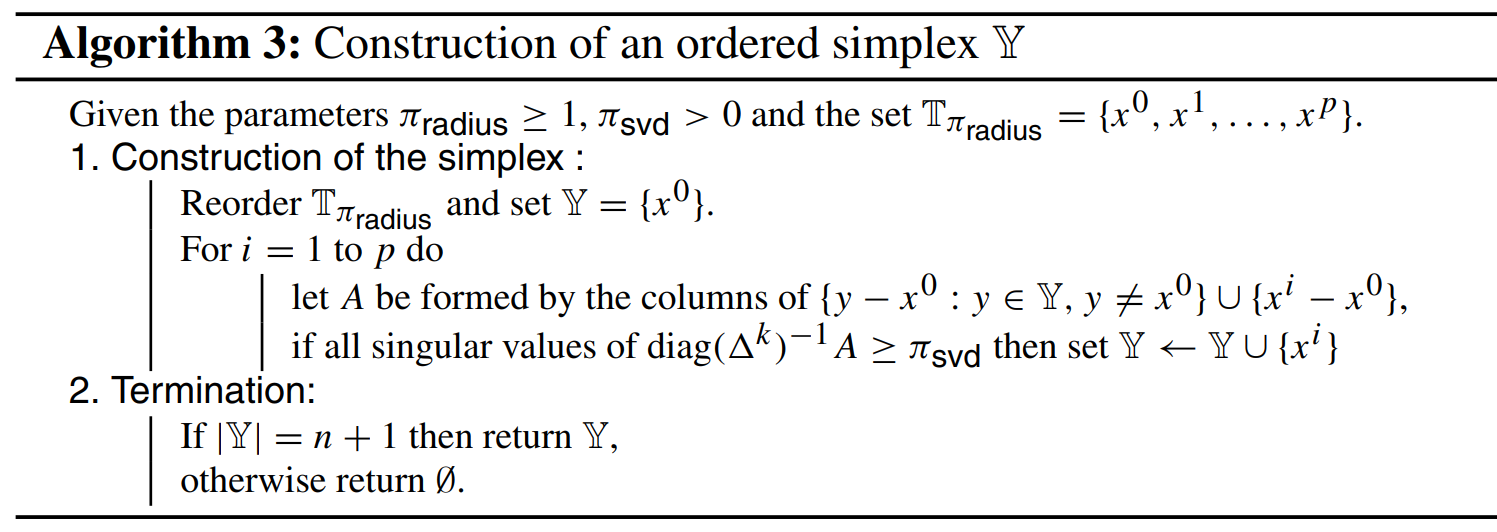
\includegraphics[width=0.8\textwidth,height=0.55\textheight]{mnm-1.png}
%  \end{itemize}
%\end{frame}

\begin{frame}{Mads-NM-基本概念}
  $$\begin{array}{ll}
    x^r_{\oplus}\quad\qquad\quad&\text{反射点 } x^r \text{舍入的网格点}\vspace{8pt}\\
    x^e_{\oplus}\quad\qquad\quad&\text{延长点 } x^e \text{舍入的网格点}\vspace{8pt}\\
    x^{oc}_{\oplus}\quad\qquad\quad&\text{外缩点 } x^{oc} \text{舍入的网格点}\vspace{8pt}\\
    x^{ic}_{\oplus}\quad\qquad\quad&\text{内缩点 } x^{ic} \text{舍入的网格点}\vspace{12pt}\\
    \mathbb{Y}^0\qquad&=\{y\in\mathbb{Y}:\not\exists x\in\mathbb{Y},\;x\prec y\}\vspace{8pt}\\
    \mathbb{Y}^n\qquad&=\{y\in\mathbb{Y}:\not\exists x\in\mathbb{Y},\;y\prec x\}\vspace{8pt}\\
  \end{array}$$
\end{frame}

%\begin{frame}{Mads-NM. constrained optimization algorithm}
%  \begin{columns}
%    \column{0.35\linewidth}
%    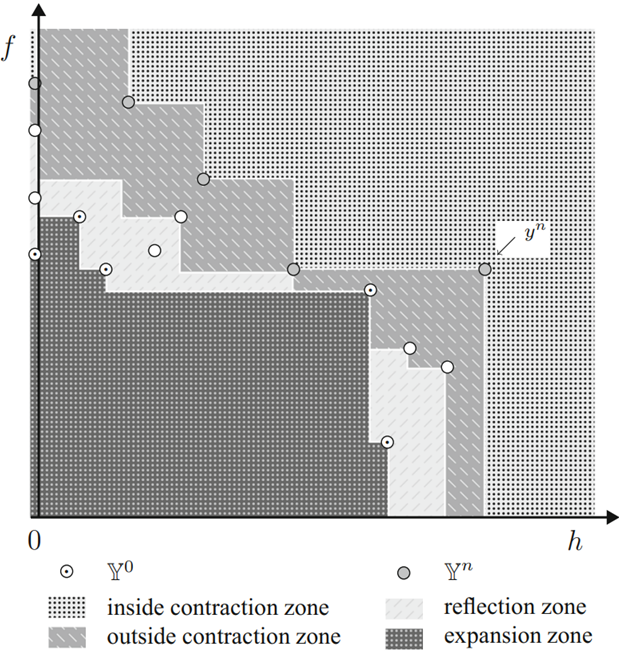
\includegraphics[width=1.1\textwidth,height=0.8\textheight]{mnm-2.png}
%    \column{0.65\linewidth}
%    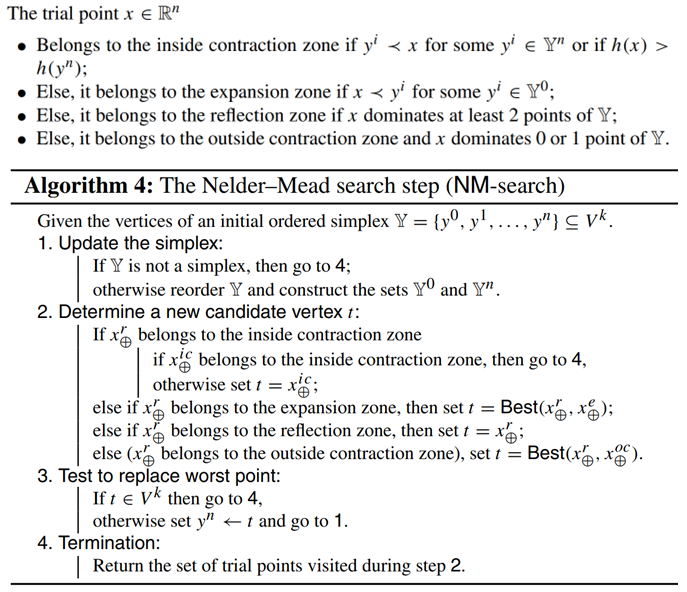
\includegraphics[width=0.9\textwidth,height=0.87\textheight]{mnm-3.png}
%  \end{columns}
%\end{frame}

\begin{frame}{Mads-NM-算法思路}
  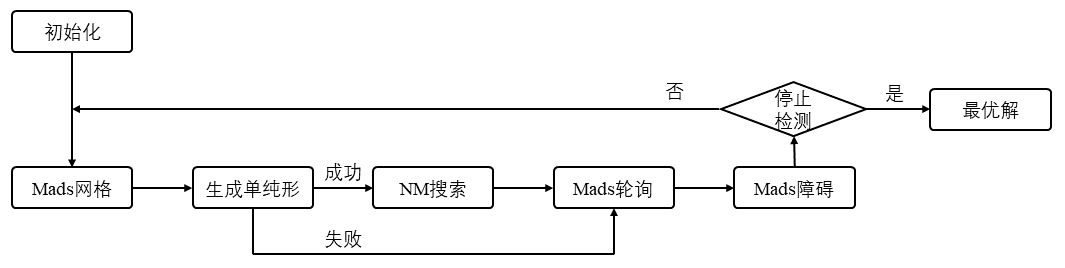
\includegraphics[width=0.95\textwidth,height=0.5\textheight]{mnm-1-c.png}
\end{frame}
%-----------------------------------------------------------------------
\section{数值实验效果比较}
\begin{frame}{调参实验}
  \begin{columns}
    \column{0.35\linewidth}
    调参实验得到参数:\vspace{30pt}

    $\begin{aligned}\pi&=(\pi_{svd},\pi_{eval},\pi_{radius})\\&=(0.01,80n,8)\\\end{aligned}$
    \column{0.6\linewidth}
    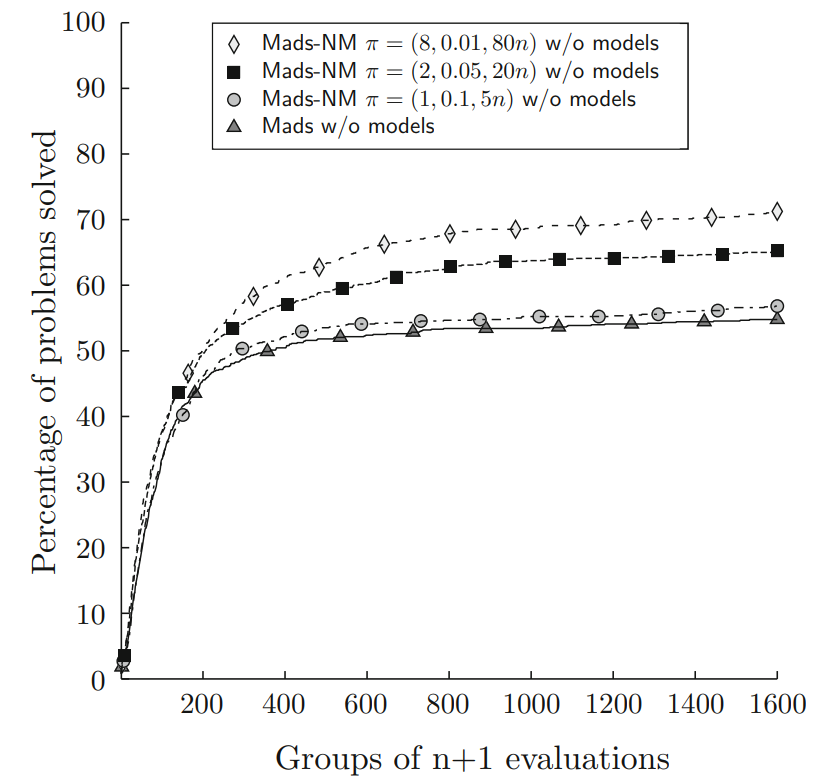
\includegraphics[width=0.8\textwidth,height=0.8\textheight]{ce-1.png}
  \end{columns}
\end{frame}

\begin{frame}{无约束问题与NM的比较}
  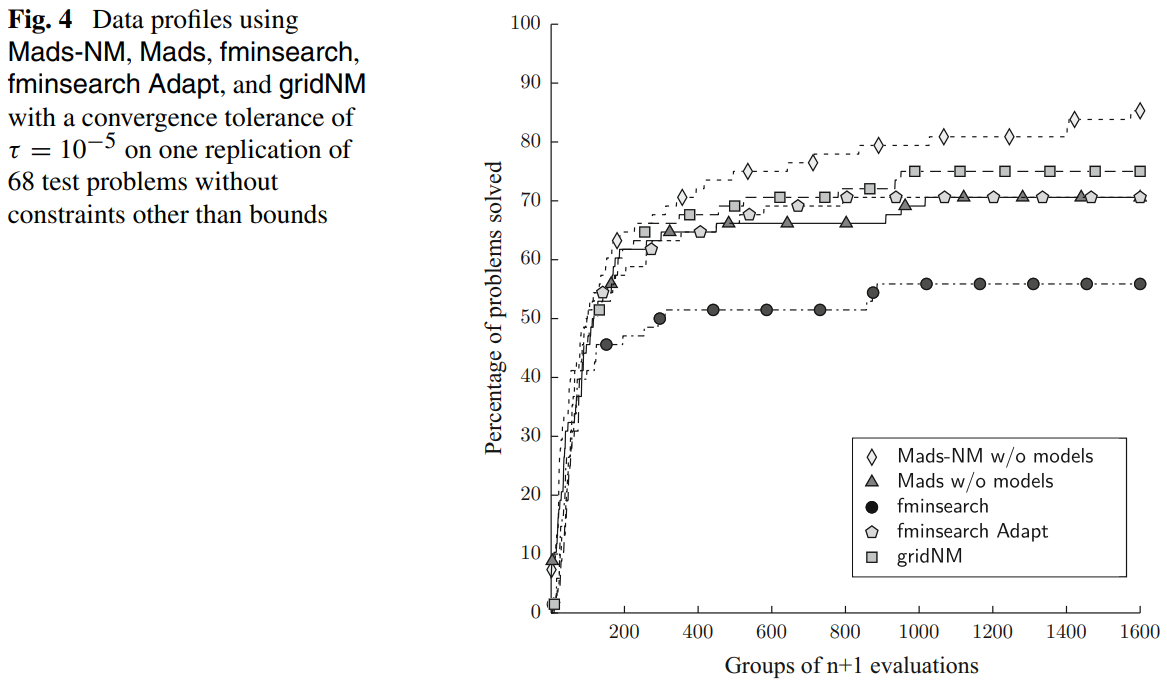
\includegraphics[width=0.8\textwidth,height=0.8\textheight]{ce-2.png}
\end{frame}

\begin{frame}{有约束问题与Mads的比较——LOCKWOOD}
  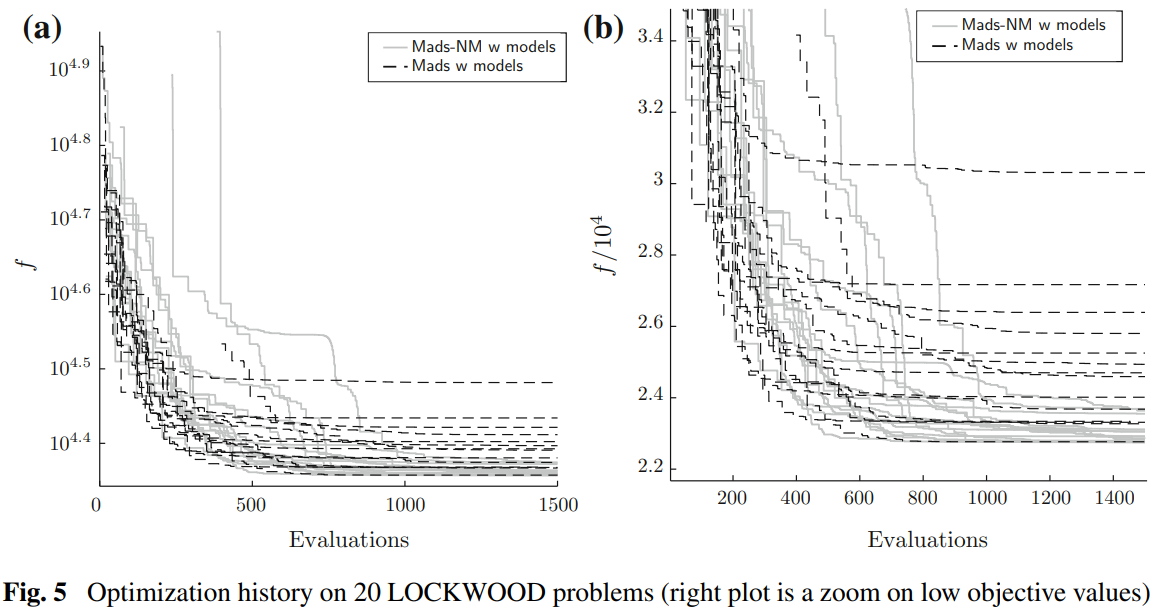
\includegraphics[width=0.8\textwidth,height=0.8\textheight]{ce-3.png}
\end{frame}

\begin{frame}{有约束问题与Mads的比较——LOCKWOOD}
  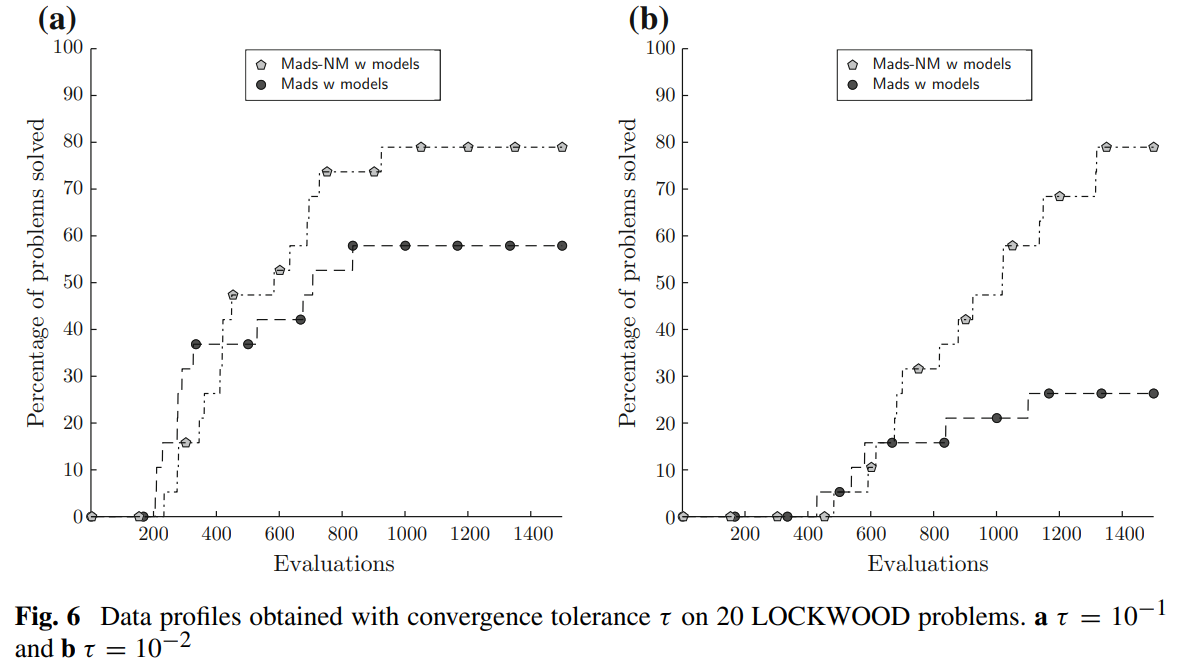
\includegraphics[width=0.8\textwidth,height=0.8\textheight]{ce-4.png}
\end{frame}

\begin{frame}{有约束问题与Mads的比较——MDO}
  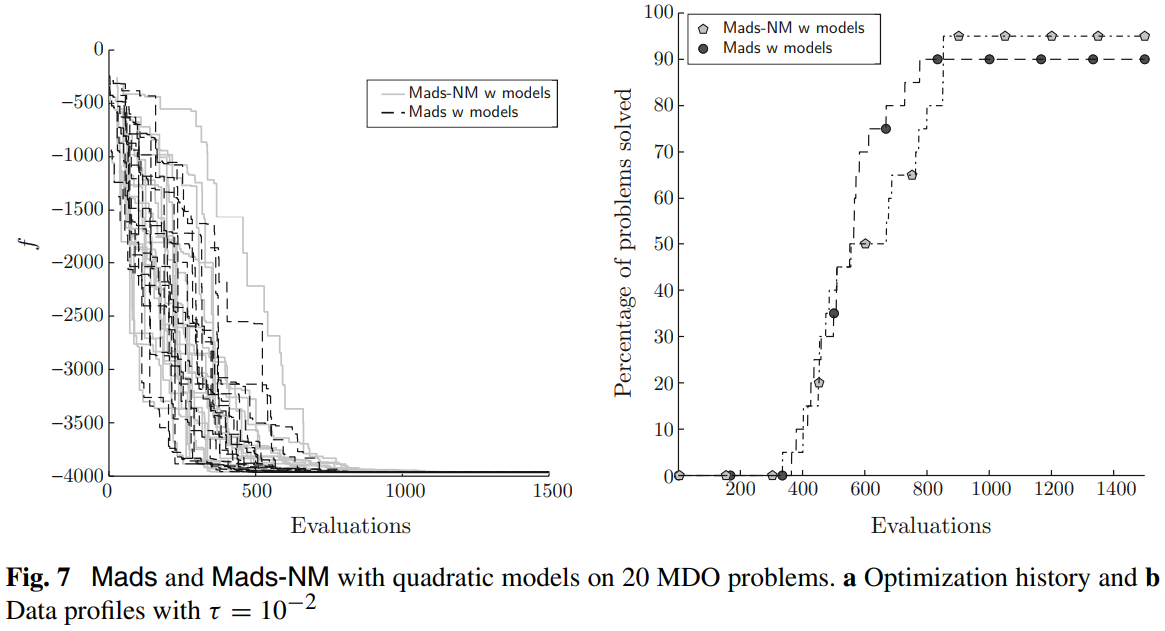
\includegraphics[width=0.8\textwidth,height=0.8\textheight]{ce-5.png}
\end{frame}

\begin{frame}{有约束问题与Mads的比较——STYRENE}
  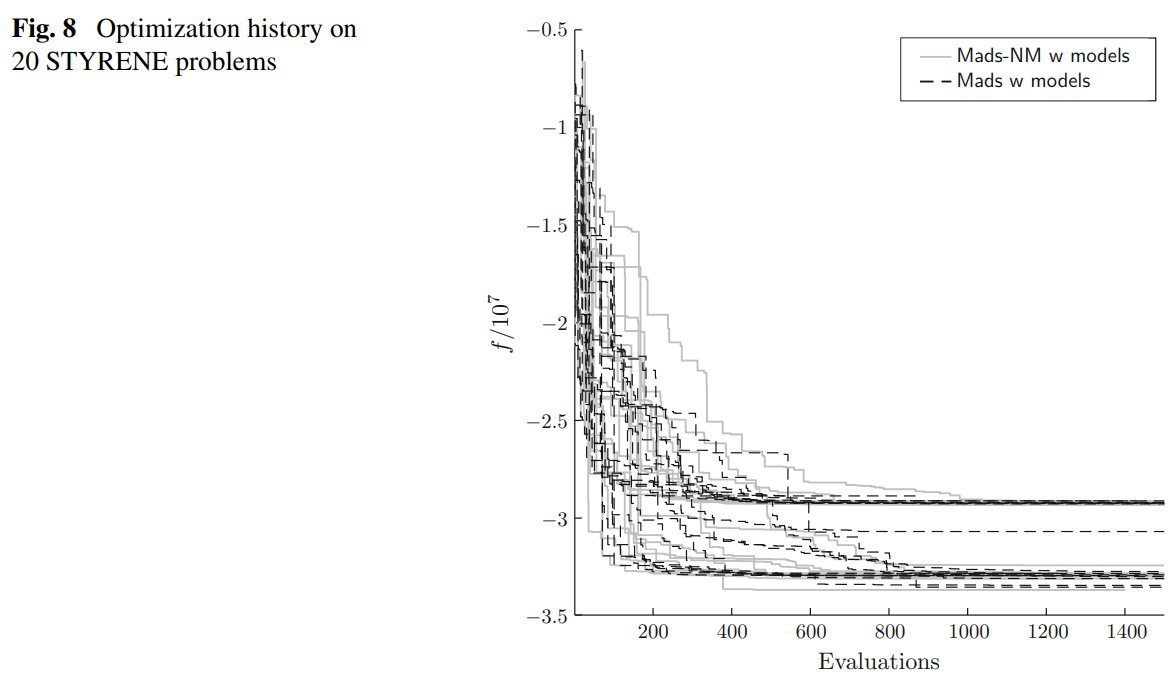
\includegraphics[width=0.8\textwidth,height=0.8\textheight]{ce-6.png}
\end{frame}

\begin{frame}{有约束问题与Mads的比较——STYRENE}
  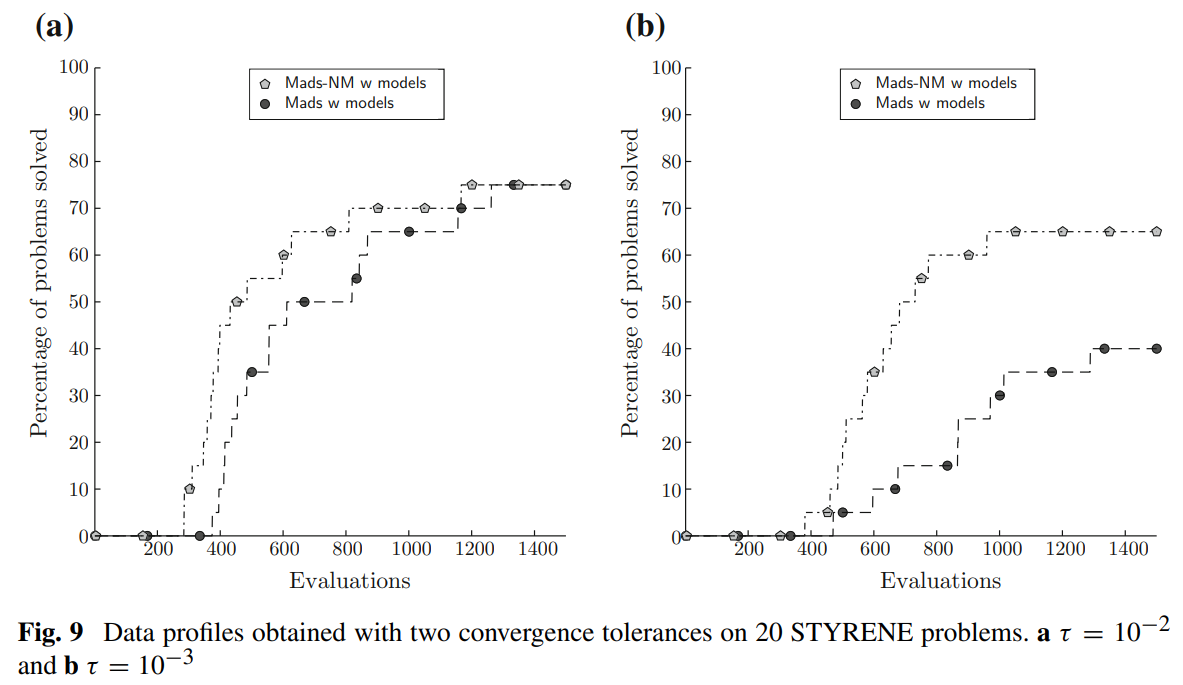
\includegraphics[width=0.8\textwidth,height=0.8\textheight]{ce-7.png}
\end{frame}
%=======================================================================
\makebottom

\end{document}
